\ylDisplay{Mutrivõti} % Ülesande nimi
{Andres Põldaru} % Autor
{lahtine} % Voor
{2015} % Aasta
{G 9} % Ülesande nr.
{8} % Raskustase
{
% Teema: Dünaamika
\ifStatement
Kui suur peab olema reguleeritava mutrivõtme keerete arv pikkusühiku kohta $n$, et mutreid saaks kõvasti kinni keerata? Hõõrdetegur kokkupuutepindade vahel on $\mu$ ja raadius reguleerija teljest kokkupuutepinnani on $r$.
\begin{center}%
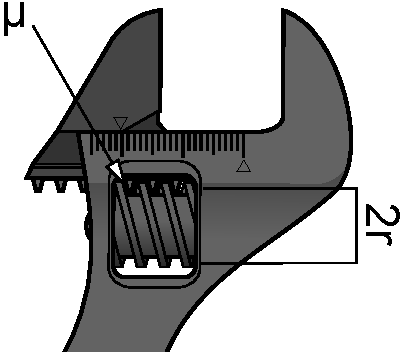
\includegraphics[width=0.4\linewidth]{2015-lahg-09-mutriv6ti_joonis}%
\end{center}
\fi


\ifHint
Esimesena on vaja leida, missugune on keermete pinnanormaali ja pöörlemistelje vaheline nurk $\alpha$. Selleks on mugav vaadelda mutrivõtme pinna jaotust. Selleks, et mutreid saaks kõvasti kinni keerata, peab hõõrdejõud tasakaalustama keermete suunas mõjuva jõu komponendi.
\fi


\ifSolution
Kui keermed on liikunud piki regulaatori telge teepikkuse $x$ võrra, on need pöördunud nurga $\varphi=2\pi nx$ võrra ning liikunud teljega risti teepikkuse $y=\varphi r=2\pi nxr$ võrra. Olgu $\alpha$ nurk pinnanormaali ja pöörlemistelje vahel. Saame 
\[
\tan(\alpha)=\frac{x}{y}=\frac{x}{2\pi nxr}=\frac{1}{2\pi rn}.
\]
Mõjugu keermetele regulaatori telje suunaline jõud $F$. Keermete suunas mõjuv jõu komponent on $F\sin\alpha$, mille peab tasakaalustama hõõrdejõud suurima võimaliku väärtusega $\mu F\cos\alpha$. Saame 
\[
\mu\geq\tan\alpha=\frac{1}{2\pi rn}
\]
ehk
\[
n\ge\frac{1}{2\pi r\mu}.
\]

\begin{center}
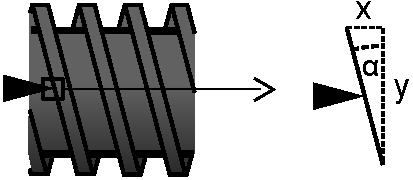
\includegraphics[width=0.5\linewidth]{2015-lahg-09-mutriv6ti_lahendus.pdf}
\end{center}
\fi


\ifEngStatement
% Problem name: Wrench
Let us take a look at a wrench that can be regulated. How big has to be the number of its grooves per unit of length, $n$, so that the nuts can be firmly fixed? The coefficient of friction between the touching surfaces is $\mu$ and the radius from the regulator’s axis to the touching surfaces is $r$.
\begin{center}%
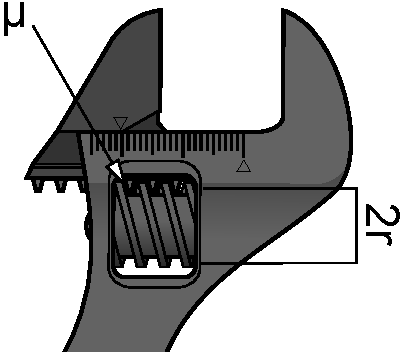
\includegraphics[width=0.4\linewidth]{2015-lahg-09-mutriv6ti_joonis}%
\end{center}
\fi


\ifEngHint
First you should find the angle $\alpha$ between the surface normal of the grooves and the rotation axis. For this it is convenient to observe the wrench’s surface development. For the nuts to be strongly fixed the friction force must balance the force component directed along the direction of the grooves.
\fi


\ifEngSolution
When the grooves have moved by distance $x$ along the axis of the regulator then they have turned by an angle $\varphi=2\pi nx$ and moved a distance $y=\varphi r=2\pi nxr$ perpendicularly to the axis. Let the angle between the surface normal and the rotation axis be $\alpha$. We get $\tan(\alpha)=\frac{x}{y}=\frac{x}{2\pi nxr}=\frac{1}{2\pi rn}$. Let there be force $F$ that has the same direction as the axis applied to the grooves. The component of the force directed along the grooves is $F\sin\alpha$, which has to be balanced by the biggest possible value of friction force $\mu F\cos\alpha$. We get that $\mu\geq\tan\alpha=\frac{1}{2\pi rn}$ meaning $n\ge\frac{1}{2\pi r\mu}$.
\begin{center}
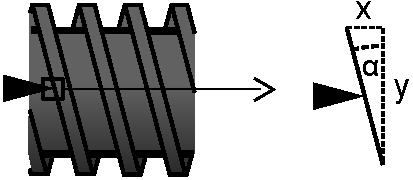
\includegraphics[width=0.5\linewidth]{2015-lahg-09-mutriv6ti_lahendus}
\end{center}
\fi
}